\documentclass[letterpaper,11pt]{article}

\usepackage[small,compact]{titlesec}
\usepackage{amsmath,bbm,amsfonts,amsthm,amssymb}
\usepackage{geometry}
\usepackage[parfill]{parskip}
\usepackage{hyperref}
\usepackage{authblk}
\usepackage{enumitem}
\usepackage{graphicx}
\usepackage[dvipsnames]{xcolor}
\usepackage{multirow,multimedia,pgfplots}
\usepackage{threeparttable,booktabs}
\usepackage{subcaption}
\usepackage{chngcntr}
\usepackage{float,lmodern}
\usepackage[backend = bibtex, style=numeric, sorting=none]{biblatex}
\usepackage[todonotes={textsize=footnotesize},authormarkup=none]{changes}
%\usepackage[final]{changes}

\hypersetup{colorlinks=true, linkcolor=cyan, filecolor=magenta, urlcolor=blue}
\urlstyle{same}
\geometry{verbose,letterpaper,tmargin=1in,bmargin=1in,lmargin=1in,rmargin=1in}


\begin{document}

% Remittances share estimation
\section{Estimate remittances sent (in \% of income)}

\begin{align} \label{eq:estim_rho}
	\rho_{od} &= \delta_1 ln(ypc_d) + \delta_2 ln(\frac{ypc_d}{ypc_o}) + \delta_3 \phi_{od} + \epsilon_{od} \nonumber \\
	ln(\rho_{od}) &= \delta_1 ln(ypc_d) + \delta_2 ln(\frac{ypc_d}{ypc_o}) + \delta_3 \phi_{od} + \epsilon_{od}
\end{align}


\paragraph{Estimation at country*country level.}
Using data on bilateral remittance flows and costs from the World Bank for 2017 (only data available for remittances):

\begin{table}[H]
%	\small
	\centering
	\begin{threeparttable}
		\begin{tabular}{lrrrrrr}
			\toprule
			                &   \multicolumn{2}{c}{remshare}   &  \multicolumn{2}{c}{ln(remshare)} \\
			\cmidrule(lr){2-3} \cmidrule(lr){4-5}
				             &      (1) &               (2) &       (3) &                  (4) \\
			\midrule
			$ypc_{o}$       & -0.020** &                   &  -0.241** &                      \\
				             &  (0.006) &                   &   (0.081) &                      \\
			$ypc_{d}$       &    0.001 &           -0.019* & -0.362*** &            -0.603*** \\
				             &  (0.004) &           (0.009) &   (0.031) &              (0.090) \\
			ypc ratio      &          &           0.020** &           &              0.241** \\
				             &          &           (0.006) &           &              (0.081) \\
			remcost ($\phi$)    &   1.276* &            1.276* &    -5.953 &               -5.953 \\
				             &  (0.616) &           (0.616) &   (3.642) &              (3.642) \\
			(Intercept)     &   0.154* &            0.154* &  3.418*** &             3.418*** \\
				             &  (0.069) &           (0.069) &   (0.831) &              (0.831) \\
			\midrule
			Estimator       &      OLS &       OLS &       OLS &       OLS  \\
			\midrule
			$N$             &   34,225 &    34,225 &     10,442 &    10,442  \\
			$R^2$        &    0.005 &             0.005 &     0.133 &                0.133 \\
			\bottomrule
		\end{tabular}
		\begin{tablenotes}
			\item *$p<0.05$, **$p<0.01$, ***$p<0.001$
		\end{tablenotes}
	\end{threeparttable}
	\caption{Estimation of remittances sent as share of migrant's income. Results from OLS regression of remittance shares (columns 1--2) and log remittance shares (columns 3--4). Dependent variables are regressed on income per capita at destination and cost of sending remittances (all columns), as well as income per capita at origin (columns 1 and 3) and ratios of destination to origin incomes (columns 2 and 4). Standard errors are clustered at the origin and destination levels.}
	\label{table:rhoest}
\end{table}


\paragraph{Estimation at region*region level.}
Using the following aggregation strategies: 
\begin{itemize}
	\item For remittance cost $\phi$: weighting corridors by remittance flows 
	\item For remittance share $\rho$: weighting corridors with weight $w_{ij}$:
		\begin{equation} \label{eq:weight}
			\forall (i,j) \in (o,d) \quad w_{ij} = \frac{stock_{ij}}{\sum_{i,j}stock_{ij}} * \frac{ypc_{mig}}{\frac{\sum_i ypc_{mig} * pop_i}{\sum_i pop_i}}
		\end{equation}
\end{itemize}

\begin{table}[H]
%	\small
	\centering
	\begin{threeparttable}
		\begin{tabular}{lrrrr}
		\toprule
		              & \multicolumn{2}{c}{remshare reg} & \multicolumn{2}{c}{ln(remshare reg)} \\
		\cmidrule(lr){2-3} \cmidrule(lr){4-5}
		              &       (1) &                  (2) &       (3) &                      (4) \\
		\midrule
		$ypc_{o,reg}$  &  -0.965** &                      & -4.957*** &                          \\
		              &   (0.306) &                      &   (0.878) &                          \\
		$ypc_{d,reg}$  & -0.573*** &            -1.538*** &   -1.579* &                -6.536*** \\
		              &   (0.102) &              (0.423) &   (0.650) &                  (0.739) \\
		ypc ratio   &           &             0.965*** &           &                 4.957*** \\
		              &           &              (0.100) &           &                  (0.878) \\
		remcost ($\phi_{reg}$)   &    2.035* &               2.035* &     9.399 &                    9.399 \\
		              &   (0.790) &              (0.790) &   (6.254) &                  (6.254) \\
		(Intercept)   &  3.490*** &             3.490*** & 11.799*** &                11.799*** \\
		              &   (0.295) &              (0.104) &   (1.609) &                  (1.609) \\
		\midrule
		Estimator     &       OLS &                  OLS &       OLS &                      OLS \\
		\midrule
		$N$           &       256 &                  256 &       251 &                      251 \\
		$R^2$         &     0.316 &                0.316 &     0.411 &                    0.411 \\
		\bottomrule
		\end{tabular}
		\begin{tablenotes}
			\item *$p<0.05$, **$p<0.01$, ***$p<0.001$
		\end{tablenotes}
	\end{threeparttable}
	\caption{See legend in Table \ref{table:rhoest}.}
	\label{table:rhoestreg}
\end{table}


\paragraph{Comparison of residuals from the two methods.} We compare residuals from equation \ref{eq:estim_rho}, more precisely $exp(\epsilon_{od})$, using:
\begin{itemize}
	\item Direct residuals of the region*region level estimation
	\item Aggregated residuals of the country*country level estimation by weighting $exp(\epsilon_{ij})$ with weigths $w_{ij}$ defined in equation \ref{eq:weight}
\end{itemize}

A comparison of residuals from both methods of estimation is displayed in Figure \ref{epsilon}.

\begin{figure}[H]
	\centering
	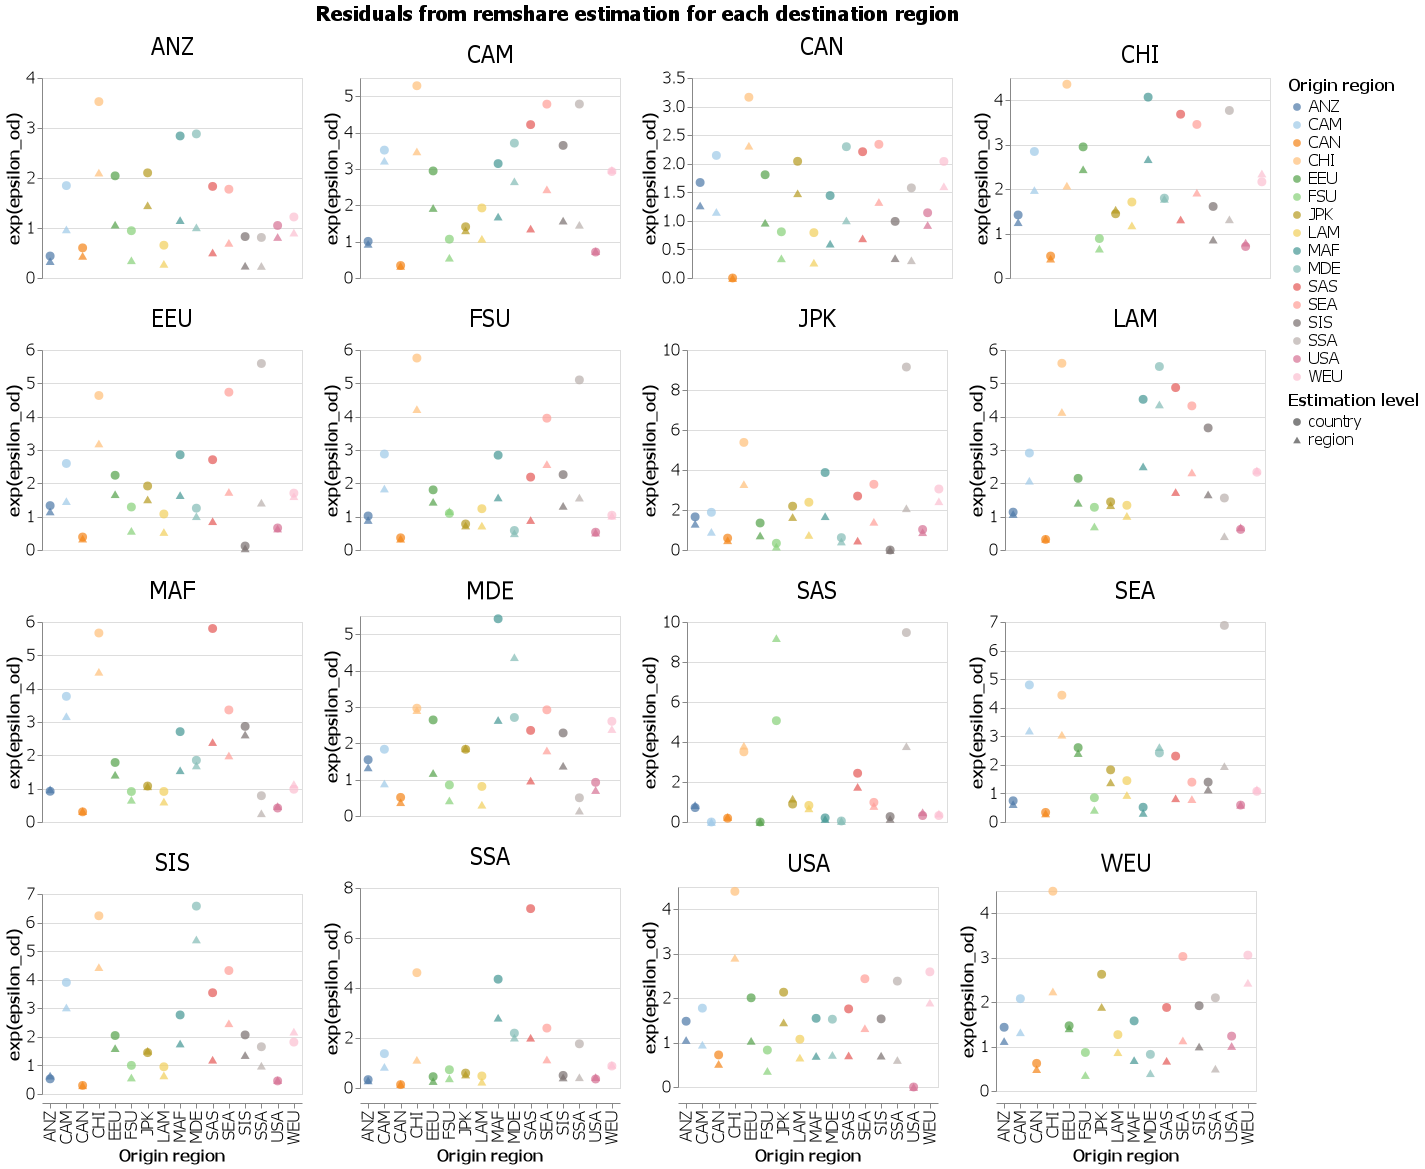
\includegraphics[width=\textwidth]{exp_epsilon_countryregion.png}
	\caption{Residuals of equation\ref{eq:estim_rho} estimating the share of income that a migrant sends back home as remittance. Residuals estimated at the country*country (circles) and region*region (triangles) level. Each of the 16 panels illustrates a destination region. The color code illustrates origin regions.}
	\label{epsilon}
\end{figure}


% Gravity estimation
\section{Estimate gravity model considering remittance shares as endogenous}

\begin{align} \label{eq:estim_grav}
	ln(move_{od}) &= ln(\beta_0) + \beta_1 ln(pop_o(t)) + \beta_2 ln(pop_d(t)) + \beta_4  ln(ypc_o(t)) + \beta_5 ln(ypc_d(t)) \nonumber \\
				&+ \beta_7 ln(dist_{od}) + \beta_8 exp(\epsilon_{od}) + \beta_9 \phi_{od} + \beta_{10} \psi_{od} + (\alpha_o + \gamma_d ) + \delta_t + \varepsilon_{odt}
\end{align}


\paragraph{Estimation at country*country level.}
Using data on bilateral migration flows from Azose and Raftery (2018) as computed in Abel and Cohen (2019) for 1990--2015, in 5-year periods; as well as residuals $\epsilon_{od}$ from equation \ref{eq:estim_rho} using specification in column (4) of Table \ref{table:rhoest}:

\begin{table}[H]
	\centering
%	\small
	\begin{threeparttable}
		\begin{tabular}{lrr}
		\toprule
		                & \multicolumn{2}{c}{migration flow} \\
		\cmidrule(lr){2-3}
		                &       (1) &                       (2) \\
		\midrule
		$pop_o$        &  0.689*** &                   0.709** \\
		                &   (0.040) &                   (0.240) \\
		$pop_d$        &  0.686*** &                  -0.722** \\
		                &   (0.042) &                   (0.238) \\
		$ypc_o$        &  0.417*** &                     0.169 \\
		                &   (0.060) &                   (0.136) \\
		$ypc_d$        &  0.830*** &                     0.010 \\
		                &   (0.070) &                   (0.096) \\
		distance        & -1.297*** &                 -1.487*** \\
		                &   (0.063) &                   (0.064) \\
		$exp(\epsilon_{od})$    &    0.011* &                    0.010* \\
		                &   (0.005) &                   (0.005) \\
		remcost  ($\phi$)      &    -9.670 &                   -12.727 \\
		                &  (15.655) &                  (15.133) \\
		comofflang ($\psi$)    &  1.743*** &                  1.591*** \\
		                &   (0.133) &                   (0.130) \\
		\midrule
		Year FE &       Yes &                       Yes \\
		Origin FE &           &                       Yes \\
		Destination FE &           &                       Yes \\
		\midrule
		Estimator       &       OLS &                       OLS \\
		\midrule
		$N$             &    73,397 &                    73,397 \\
		$R^2$           &     0.479 &                     0.611 \\
		Within-$R^2$    &     0.478 &                     0.366 \\
		\bottomrule
		\end{tabular}
		\begin{tablenotes}
			\item *$p<0.05$, **$p<0.01$, ***$p<0.001$
		\end{tablenotes}
	\end{threeparttable}
	\caption{Estimation of gravity model. Results from OLS regression of migration flows. Specifications with year fixed effects (all columns), and origin and destination fixed effects (column 2). Estimates are obtained based on data from Azose and Raftery (2018) as computed in Abel and Cohen (2019). Intercept computed as constant plus average values of year fixed effects. Standard errors are clustered at the origin and destination levels.}
	\label{table:gravest}
\end{table}


\paragraph{Estimation at region*region level.}
Using the same data, and the following aggregation strategies: 
\begin{itemize}
	\item For distances $dist$: distances between centers of population of regions, computed as aryhtmetic means of coordinates of a region's countries' capitals weighted by population
	\item Direct residuals of the region*region level estimation from equation \ref{eq:estim_rho} using specification in column (4) of Table \ref{table:rhoestreg}
	\item For remittance cost $\phi$: weighting corridors by remittance flows 
	\item For common offficial language $\psi$: weighting corridors by migrant flows
\end{itemize}

\begin{table}[H]
	\centering
%	\small
	\begin{threeparttable}
		\begin{tabular}{lrr}
		\toprule
		                & \multicolumn{2}{c}{migration flow} \\
		\cmidrule(lr){2-3}
		                &       (1) &                       (2) \\
		\midrule
		$pop_o$        &    0.676 &            1.226 \\
		                &  (0.879) &          (0.935)  \\
		$pop_d$        &    0.524 &         1.581*** \\
		                &  (2.767) &          (0.449) \\
		$ypc_o$        &    0.895 &            0.429 \\
		                &  (0.512) &          (0.371) \\
		$ypc_d$        &    1.427 &            0.473 \\
		                &  (1.119) &          (1.279) \\
		distance         &   -0.711 &           -0.680 \\
		                &  (4.348) &          (0.562) \\
		$exp(\epsilon_{od})$      &   -0.293 &           -0.190 \\
		                &  (1.364) &          (0.278) \\
		remcost  ($\phi$)        &   14.647 &           -1.379 \\
		                &  (8.950) &          (3.933) \\
		comofflang ($\psi$)    & 2.183*** &            0.504 \\
		                &  (0.322) &          (0.461) \\
		(Intercept) & -32.122 & -0.008  \\
		\midrule
		Year FE &       Yes &                       Yes \\
		Origin FE &           &                       Yes \\
		Destination FE &           &                       Yes \\
		\midrule
		Estimator       &       OLS &                       OLS \\
		\midrule
		$N$             &    1,170 &            1,170   \\
		$R^2$           &   0.559 &            0.797  \\
		Within-$R^2$   &    0.556 &            0.471 \\
		\bottomrule
		\end{tabular}
		\begin{tablenotes}
			\item *$p<0.05$, **$p<0.01$, ***$p<0.001$
		\end{tablenotes}
	\end{threeparttable}
	\caption{See legend in Table \ref{table:gravest}.}
	\label{table:gravestreg}
\end{table}


\paragraph{Comparison of residuals from the two methods.} We compare residuals from equation \ref{eq:estim_grav}, more precisely $move_{od} - \hat{f}_{grav}(...)$. A comparison of residuals from both methods of estimation is displayed in Figure \ref{residual}.

\begin{figure}[H]
	\centering
	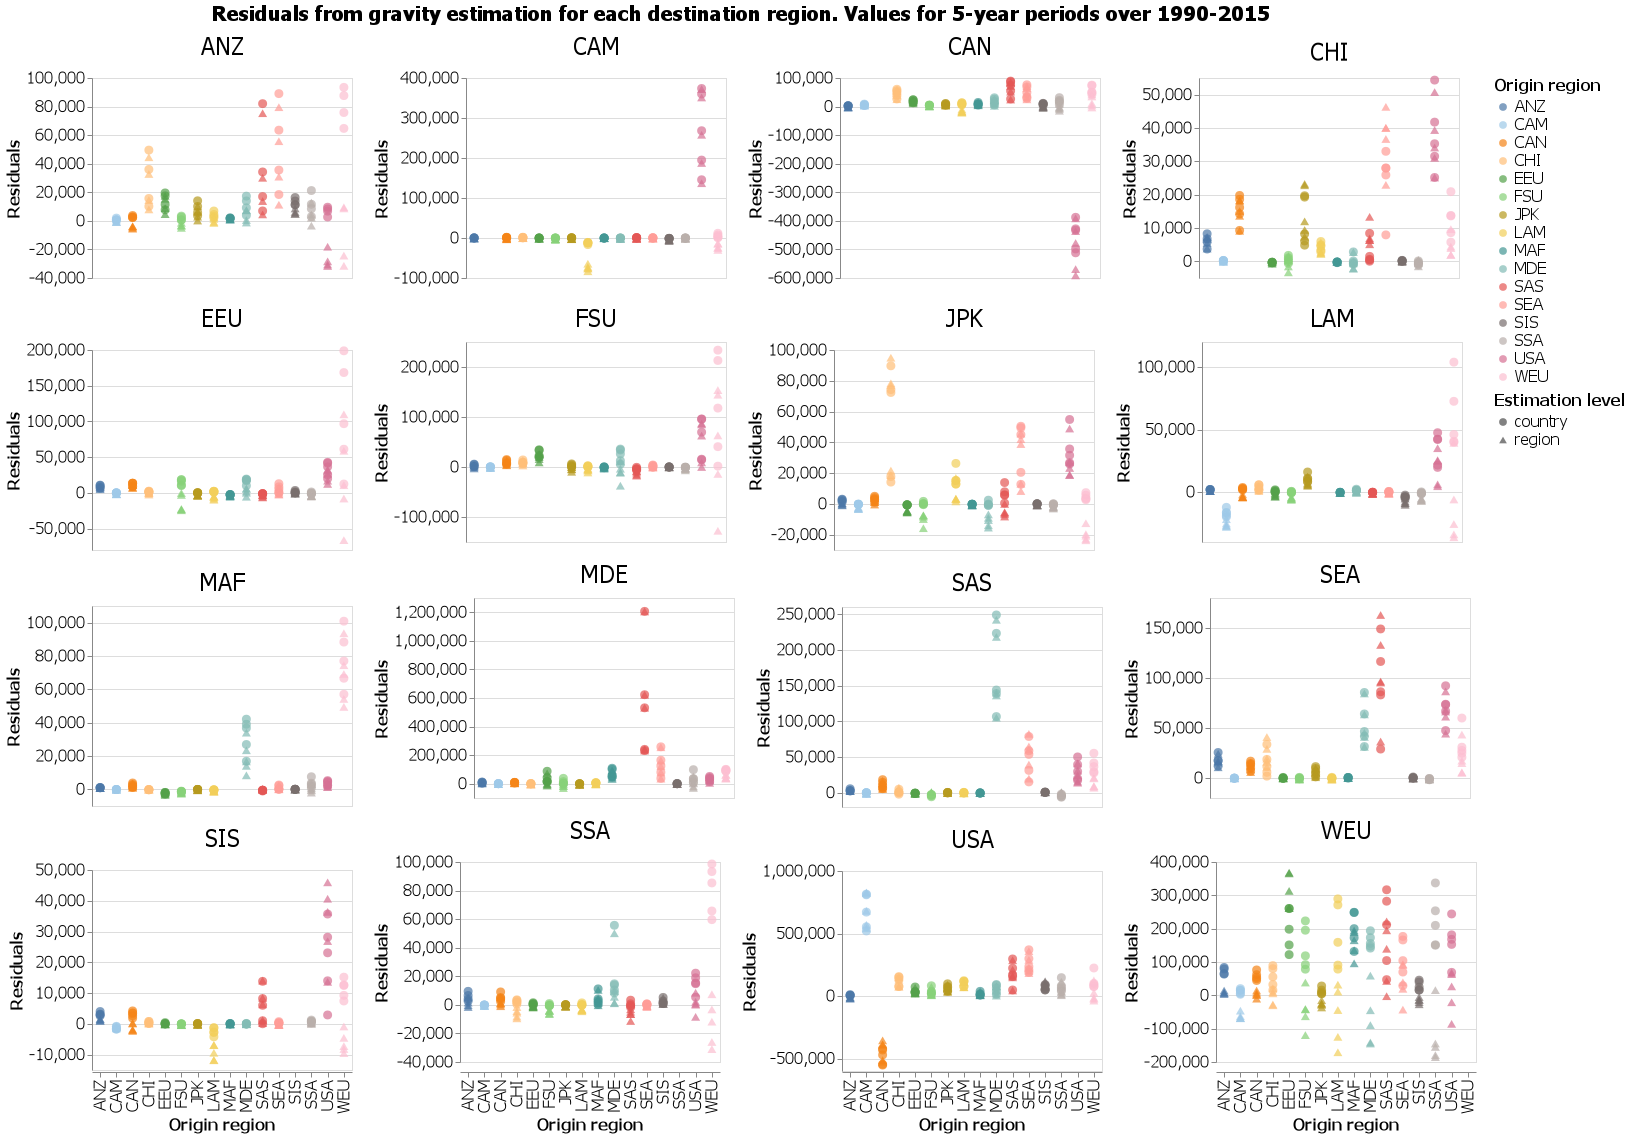
\includegraphics[width=\textwidth]{residuals_countryregion.png}
	\caption{Residuals of equation \ref{eq:estim_grav} estimating the number of people moving between two regions following our gravity model. Residuals estimated at the country*country (circles) and region*region (triangles) level. Each of the 16 panels illustrates a destination region. The color code illustrates origin regions. Values from five 5-year periods, spanning 1990-2015, are presented.}
	\label{residual}
\end{figure}

\end{document}